\documentclass{article}
\usepackage{enumitem}
\usepackage{amsmath}
\usepackage{graphicx}
\begin{document}
\title{T-Flipflop}
\begin{enumerate}
	\item Two T-flip flops are interconnected as shown in the figure. The present state of the flip flops are: $A = 1, B = 1$. The input x is given as $1, 0, 1$ in the next three clock cycles. The decimal equivalent of $(ABy)_{2}$ with A being the MSB and y being the LSB, after the 3\textsuperscript{rd} clock cycle is \rule{12mm}{0.4pt}
	\begin{figure}[ht]
		\centering
			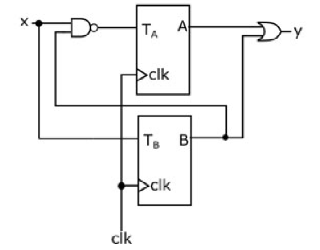
\includegraphics[width=\columnwidth]{figs/cktdiag.png}
		\caption{}
		\label{fig:cktdiag}
	\end{figure}
\end{enumerate}
\end{document}
